\section{Results}

Our experiment measured the eye and body movements as subjects performed a sorting task in a virtual environment. The participants sorted objects based on the color and/or shape where we modulated the task complexity into EASY and HARD trials. We further divided the trials into planning and execution epochs where subjects  planned the selection of the target objects to interact with and then executing the action of displacing it to target shelves, respectively. In this section, we report the behavioral differences of the subjects for the two task types (EASY, HARD), the scan-path differences in the planning and execution epochs and finally the timing of the first fixations on regions-of-interest based on the action sequences.

\subsection{Task based Behavioral Differences}
In the present study, the primary object related action was to repeatedly pickup objects and place them at a desired locations until they are sorted according to the sorting task. \textcolor{Blue}{Figure \ref{figure:easy_hard_diff_1}} shows the differences in EASY and HARD trials based on the time taken to finish the sorting task. The EASY trials require sorting the objects based on a single feature, the trial duration is shorter (Mean=56.02 seconds, SD=23.308) as compared to HARD trials (Mean=132.16 seconds, SD=116.18) where subjects had to sort taking into account both features (color and shape) of the objects. 

In order to compare the experimental object displacements for the two trial type, we also designed a depth-first search algorithm that computed the minimum number of displacements required to sort the objects for the 5000 random configurations of 16 objects in 25 shelf locations for both EASY and HARD trials. \textcolor{Blue}{Figure \ref{figure:easy_hard_diff_2}} shows the comparisons in the object displacements made by the subjects and the optimal number of displacements as elicited by the search algorithm for both EASY and HARD trials. Subjects made lower number of object displacements in the EASY trials (Median=10, IQR=[8, 13]) compared to HARD trials (Median=15, IQR=[11, 20]). In the EASY trials subjects performed closely with the optimal search algorithm (Median=9, IQR=[9,10]), whereas, in the HARD trials, subject were more sub-optimal compared to the algorithm (Median=11, IQR=[9,13]).

\begin{figure}[h]
    \centering
    \subfloat[][]{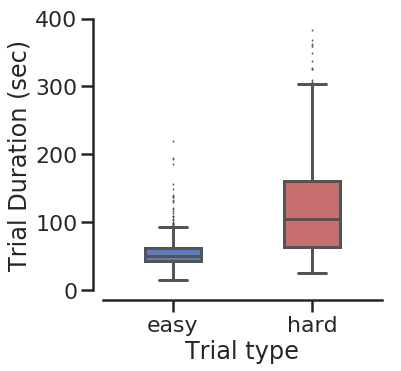
\includegraphics[width=0.25\linewidth]{source/figures/results/TrialDuration.png} \label{figure:easy_hard_diff_1}}
    \hspace{2cm}
    \subfloat[]{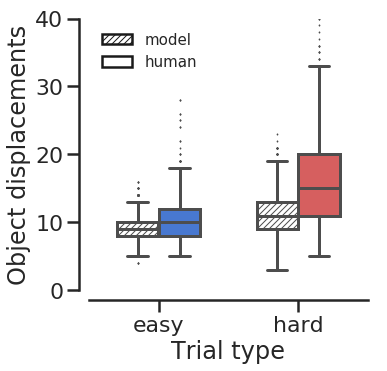
\includegraphics[width=0.25\linewidth]{source/figures/results/grasps.png} \label{figure:easy_hard_diff_2}}
    \caption{Behavioral differences based on the 2 tasks: \protect\subref{figure:easy_hard_diff_1} Trial duration of the EASY and HARD trials. The boxplots show the inter-quartile range (IQR) of the duration of the trials for the two different trial types for all trials and participants. The whiskers represent 1.5 times the IQR. The median duration for the EASY trials was 60 seconds while 110 seconds for HARD trials.\protect\subref{figure:easy_hard_diff_2} Distribution of number of object displacements for EASY (blue) and HARD (red) trials. The colored box plots show the inter-quartile range of the number of object displacements made by subjects per trial and per participant. The whiskers represent 1.5 times the IQR. The dashed box plots show optimal number of displacements required to sort the objects for a model computed with a depth-first search algorithm for 5000 random trial initialization for each trial type.
    }
\end{figure}

Next, to check the propensity to pickup and drop-off objects from and to preferred locations on the shelf, we plotted the density of pickup locations and drop-off locations in \textcolor{Blue}{Figure \ref{figure:obj_displacement}}. Given the sorting tasks where subjects were presented with random initial configurations of the objects on the shelf locations, we did not expect any systematic spatial biases at play. Further, the expectation was that the subjects would move the objects randomly and not display a preference for object pickup and drop-off locations. As seen in \textcolor{Blue}{Figure \ref{figure:pick_up}} at the start of the moving of the object, in the case of easy trials objects are preferentially picked up from the the rightmost column and bottom row of the shelf. Conversely, for the hard tasks the objects are picked up from all locations and there is no systematic preference for the pickup location on the shelf. Interestingly, for both EASY and HARD trials, subjects did not move the objects from the top and left-most locations of the shelf. Secondly, as seen in  \textcolor{Blue}{Figure \ref{figure:drop_off}} subjects show a propensity to drop the objects leaving out the right column and bottom row of the shelf for both EASY and HARD trials. 

This shows that subjects systematically, displace the objects leftward and upward employing an arbitrary heuristic to complete both task types. As the objects are instantiated on the shelf randomly, an optimal strategy would not show this behavior. We can conclude from the above that subjects offset their cognitive load of optimally completing the task by employing simple heuristics. Further, this behavior can also be explained as a way to reduce the physical effort and make ergonomic compensations by placing all objects at a higher ground level in order to bend the body fewer times during the task. In other words, in lieu of optimally performing the task and finishing it in a shorter time, subjects prefer to offload both cognitive and physical effort on the environment by adopting a more sub-optimal strategy.

\begin{figure}[h]
    \centering
    \subfloat[]{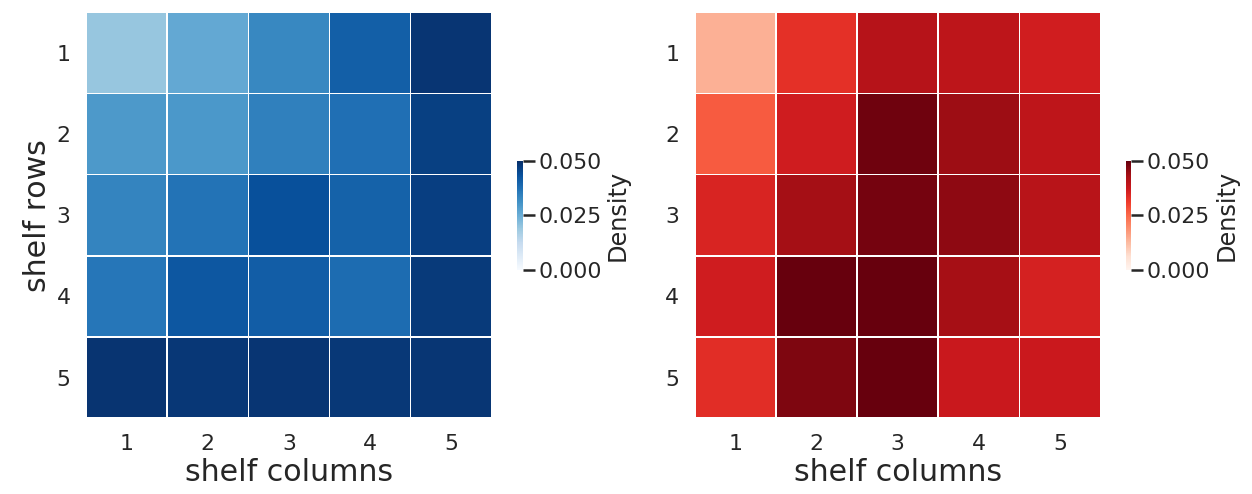
\includegraphics[width=0.55\linewidth]{source/figures/results/shelf_grasp_pickup_locations.png}
     \label{figure:pick_up}}\\
    \subfloat[]{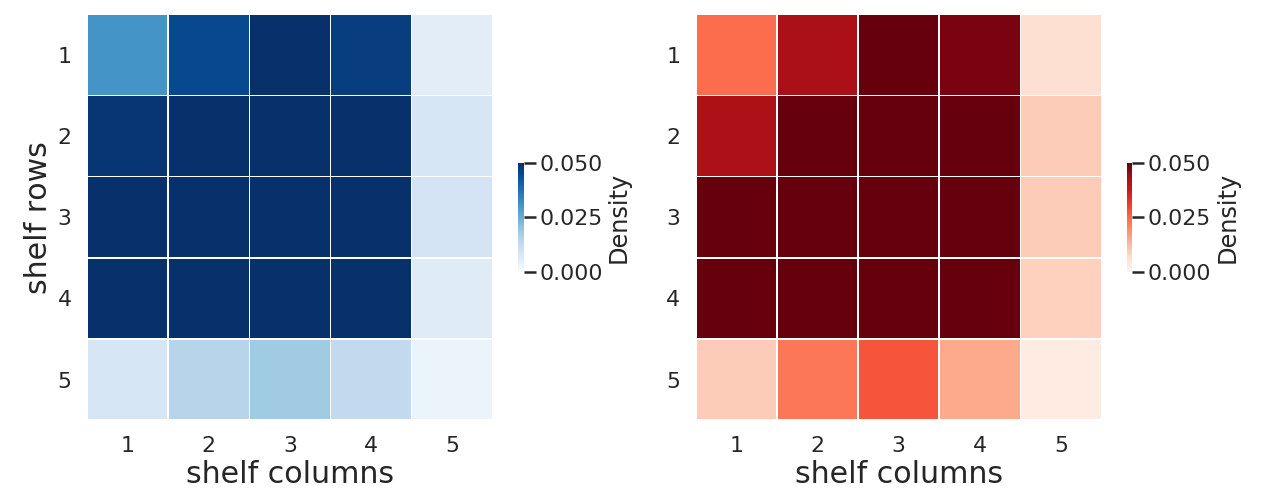
\includegraphics[width=0.55\linewidth]{source/figures/results/shelf_grasp_drop_locations.png}
     \label{figure:drop_off}}\\
    \caption[]{Object displacement behavior for 60 subjects and 16,500 displacements made over all shelf 5x5 locations with blue heatmaps showing probability density over EASY trials and red heatmaps showing density over HARD trials. \protect\subref{figure:pick_up} shows the probability density at the start of each object displacement. This indicates that subjects have a propensity to pickup objects from the rightmost column and bottom column for EASY trials (left) and conversely, in the HARD trials (right) subjects pickup objects from central locations. For both trial types, objects in the top-left corner of the shelf are not picked up. \protect\subref{figure:drop_off} shows the probability density at the end of the object displacement. This indicates that for both EASY (blue, left) and HARD (red, right) trials, subjects display a systematic propensity to place the objects every where other than the bottom row or rightmost column. }
    \label{figure:obj_displacement}
\end{figure}

\subsection{Role of Eye Movements in Action Execution \& Planning}

In this section, we investigate the role of eye movements specific to action planning and execution. The action of picking up an object and dropping it to a shelf location requires precise attention on the object to be grasped and then a shift of gaze to the location of the place where the object will be dropped off. The change of proportion of fixations on the task-relevant objects of interest over time would reveal the average shift of gaze before and during the action execution. To do this, we employ seven regions-of-interest for each action of displacing an object. These regions-of-interest consist of the current target object (current\_TO) that is being displaced, the current target shelf (current\_TS) where the object is displaced finally, the previous target object (prev\_TO) and previous target shelf (prev\_TS) that were relevant in the previous action, the next target object (next\_TO) and next target shelf (next\_TS) that will be interacted with in the next action in the sequence, and finally all the other objects and shelves that were not relevant in the action sequence. We selected the 3s before the virtual hand touches the object (grasp onset) and 3s after and divided it into 0.25 second bins to calculate the proportion of fixations on all of the ROIs within each time bin. Hence, we can assess the dynamic changes in the proportion of fixations on the seven ROIs as the current action is planned and executed.

\begin{figure}[h]
    \centering
    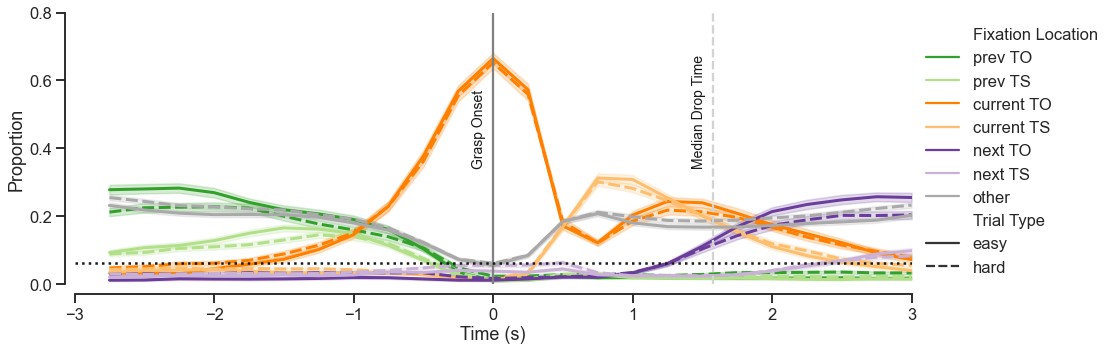
\includegraphics[width=0.9\linewidth]{source/figures/results/time_course_proportion_7ROI.png}
    \label{figure:timecourse_fixprop}\\
    % \subfloat[]{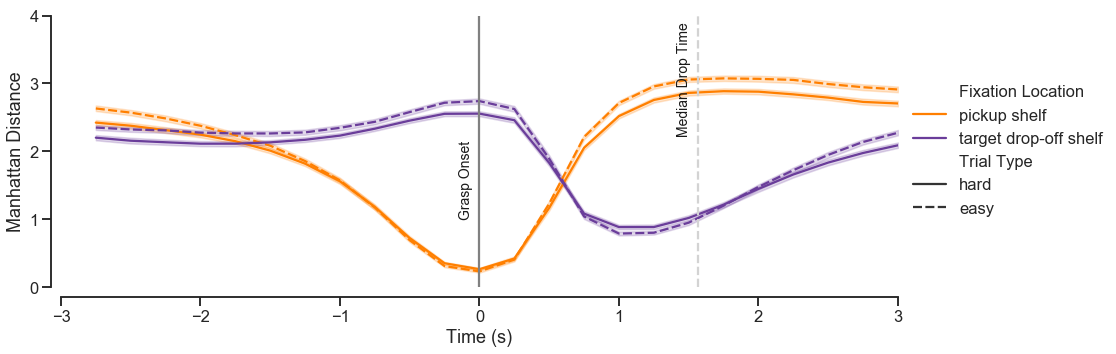
\includegraphics[width=0.7\linewidth]{source/figures/results/time_course_fix_distance.png}
    % \label{figure:timecourse_manhattan}}
    \caption[]{ Time course of proportion of fixations centered on the object displacement initiation (grasp onset) at time=0 and 3 seconds before and after on the seven regions of interest and for the two trial types (EASY and HARD). The black dotted horizontal line indicate the chance level (1/16)  of fixating on a target object. The shaded regions show 95\% confidence interval of the mean proportion of gaze at each time-bin across all trials within a trial type. These regions-of-interest consist of the current target object (current\_TO) that is being displaced, the current target shelf (current\_TS) where the object is displaced finally, the previous target object (prev\_TO) and previous target shelf (prev\_TS) that were relevant in the previous action, the next target object (next\_TO) and next target shelf (next\_TS) that will be interacted with in the next action in the sequence, and finally all the other objects and shelves that were not relevant in the action sequence.
    % Panel \protect\subref{figure:timecourse_manhattan} Time course of Manhattan distance (city-block distance) of fixations on the shelf from the pick-up location at start of object displacement and drop-off location at end of object displacement. The time-course is epoched from 3 seconds before grasp onset at time=0 seconds and 3 seconds after. The shaded regions show 95\% confidence interval of the mean manhattan distance of gaze at each time-bin.
   }
    \label{figure:timecourse}
\end{figure}

As a first step, we wanted to study the average oculomotor profiles across time over the seven ROIs and the trial types. The average profile will reveal any systematic gaze shifting strategy from previous, to current and then to next in the action sequence. \textcolor{Blue}{Figure \ref{figure:timecourse}} shows the time course of proportion of fixations on the seven ROIs as described above for the two task types. We can see that proportion of fixations on the current target object are above chance level (1/16) at approximately 2 seconds before grasp onset with maximum proportion of fixations on the target object at the time of grasp onset. Before grasp onset, the average profile reveals equal proportion of fixations on the previous target object and other regions on the shelf. As the fixations on the previous target object and shelf decrease, the fixations on the current target object increase monotonically and are maximum at the grasp onset. Throughout the period before the grasp onset, gaze on the next target object and shelf remains below chance level. After the grasp is initiated, the gaze shifts from the current target object and goes to the current target shelf where the proportion of fixations on the target shelf and non-target other ROI increases monotonically and is maximum approximately 1 second after grasp onset. Moreover, the average proportion of fixations for the 'other' ROI is consistently low during the action execution and only increase once the action is completed. Moreover, we see that before the median end of the action at 1.64 seconds after the grasp onset, the fixations are above chance level on the next target object. The presence of fixations on the next target object even before the end of the current action execution indicates, that the next action is queued in for execution shortly before ending the current action. Also, as there are no significant differences in the fixation probabilities on the ROIs across time for the two trial types, we can conclude that this oculomotor behavior is purely related to action execution and is not affected by the cognitive load of the different sorting tasks. Most importantly, we see that the fixations are made in a just-in-time manner with the gaze shifting systematically in sync with the previous, current and next action sequence one after the another. This indicates that the oculomotor system is engaged in a just-in-time manner for the sub-actions of picking up and dropping off one after the other.

The above results, illustrate the average spatial and temporal aspects of attention during action execution. However, the scanning behavior of subjects while they perform each action is "averaged out" with this technique. In order to study the scanning behavior while subjects plan and execute an action, we computed transition matrices to capture fixations to and from each of the seven ROI. The ROIs used are described in Section 2.5. With the transition matrices we wanted to capture the gaze guidance behavior of the subjects while they plan and execute the actions. The relative net-transitions within the planning and execution epochs of a trial tell us the gaze guidance behavior of the subjects during those epochs. With higher relative net transitions, we expect higher gaze guidance to the task-relevant ROIs, i.e, subjects do not necessarily search for the best action for the task. If subjects perform a search and fixate on multiple ROIs indiscriminately within an epoch, we would expect lower relative net transitions indicating a pattern of fixations related to planning the best (most optimal) actions. 

\begin{figure}[h]
    \centering
    \subfloat[]{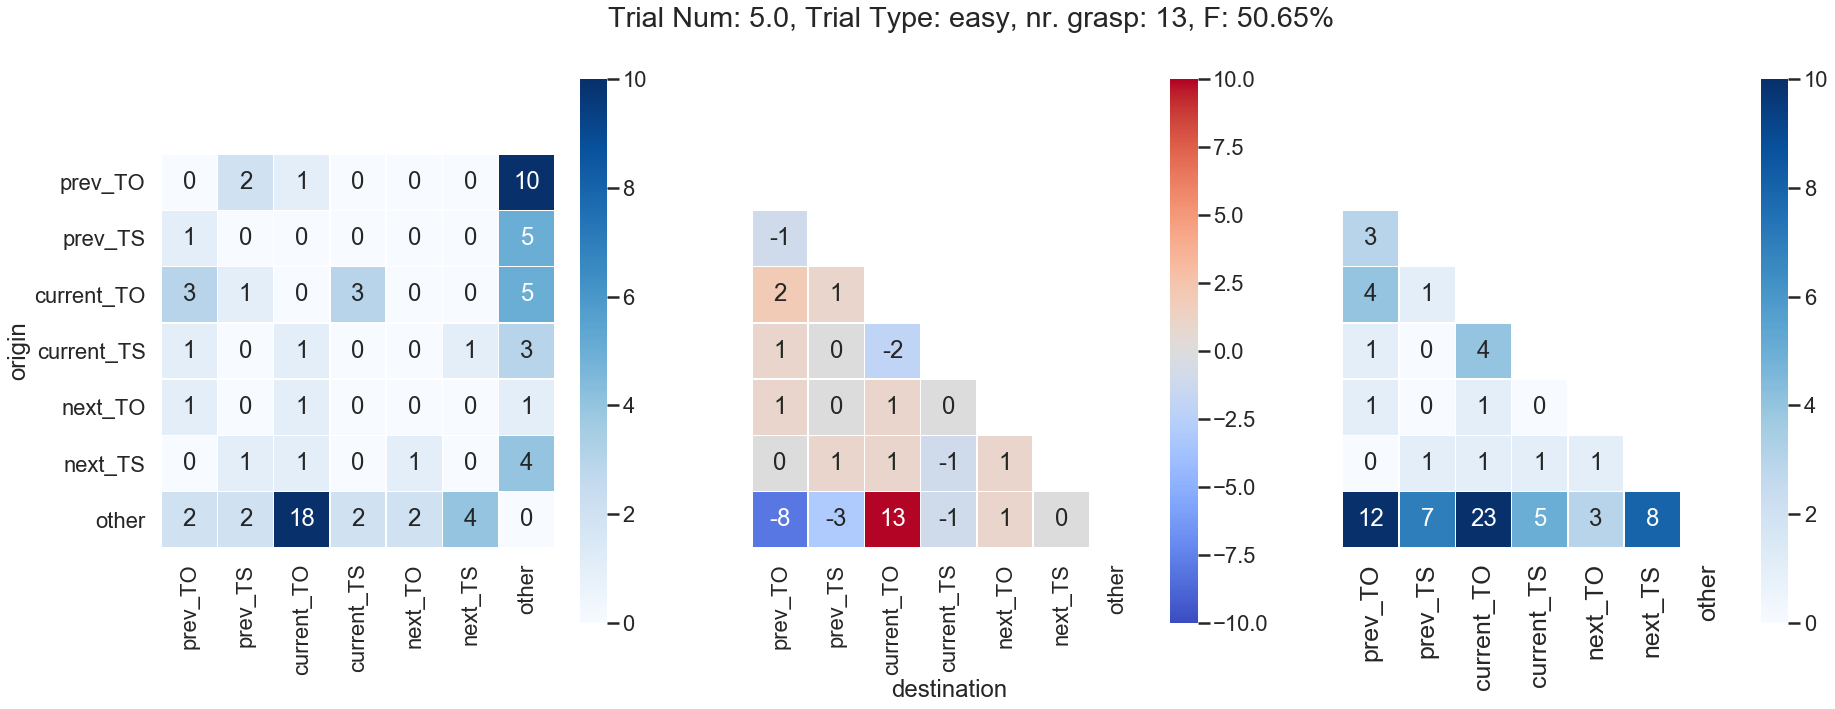
\includegraphics[width=0.7\linewidth]{source/figures/results/transition_matrix_trial_5.png}
    \label{figure:transition_1}} \\
    \subfloat[]{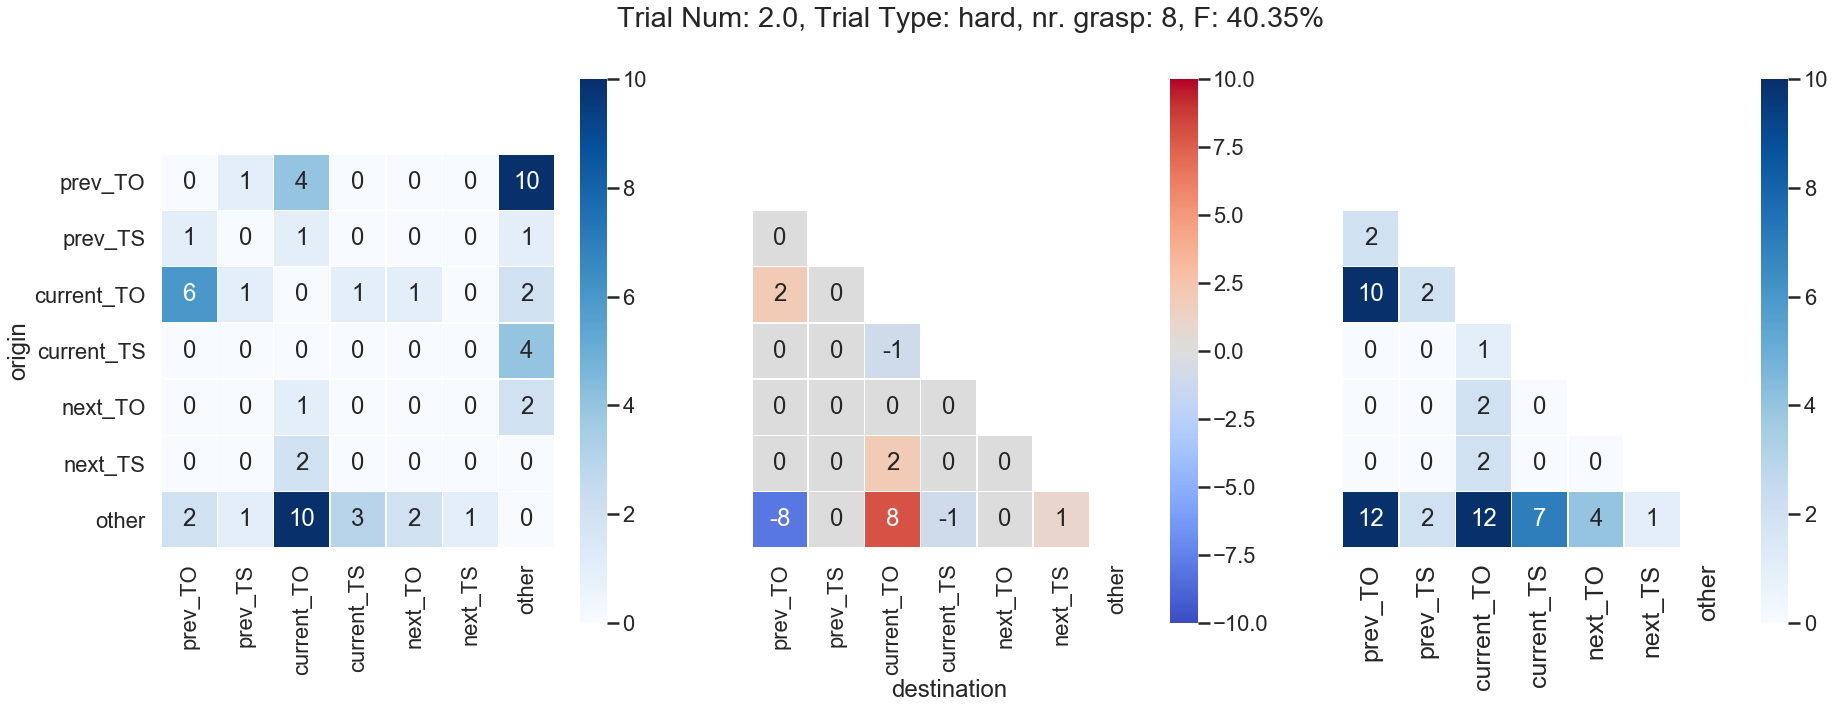
\includegraphics[width=0.7\linewidth]{source/figures/results/transition_matrix_trial_2.png}
    \label{figure:transition_2}}
    \caption[]{Exemplar transition matrices for gaze switching between end of previous grasp and start of current grasp for the two trial types. The ordinate defines the origin of the gaze i.e. where the gaze was before and the abscissa defines the destination of the gaze. The diagonal contains zero as the transition is defined as a saccade from one region of interest to another. In this example there are 7 regions of interest.They are defined here as the previous target object and shelf (prev\_TO, prev\_TS), the current target object and shelf (current\_TO, current\_TS) that are manipulated in the current epoch and the next target object and shelf (next\_TO, next\_TS) that will be used in the next grasping epoch. All other objects and shelf locations that are not specific to the above regions of interest are defined as 'other'. The left panel shows the transition matrix, A. The middle panel, shows the net transitions (A\textsubscript{NET}) to the regions of interest. The positive number in the matrix denotes transitions from source ROI to destination ROI, whereas the negative numbers reverse the direction of transition and denote the transition away from destination to source. The right panel shows the total transitions (A\textsubscript{TOTAL})  made between the 7 regions of interest. The F value in the in the figure title refers to the relative number of transitions in the net transition matrix.\\
    Panel \protect\subref{figure:transition_1} shows the transition matrix of a given trial for the gaze switching in an EASY trial with 13 grasps/object displacements. As shown in the middle panel, in the trial, 8 transitions are made from prev\_TO to other, whereas 13 transitions are made from 'other' to current\_TO. The right panel shows the total number of transitions made between the ROIs. This tells us the that a majority of the transitions are from 'other' sources to the regions of interest. The F value for this trial shows that 50.65\%  net transitions explain the total transitions.\\
    Panel \protect\subref{figure:transition_2} shows the transition matrix for the gaze switching of a given trial in a HARD trial with 8 grasps/object displacements. As shown in the middle panel, in the trial, 8 transitions are made from prev\_TO to other, and 8 transitions are made from 'other' to current\_TO. And other ROI have close to net zero transitions. The right panel shows the total number of transitions made between the the ROIs. This tells us the that a majority of the transitions are from 'other' sources to the regions of interest. The F-value for this trial shows that 40.35\%  net transitions explain the total transitions.}
    \label{figure:transition_matrices_plan}
\end{figure}

\textcolor{Blue}{Figure \ref{figure:transition_matrices_plan}} shows the exemplar transition matrices, net transitions and total transitions for an  EASY and HARD trial. The matrices capture the gaze switches from and to the 7 ROIs taking together all the action planning epochs in a trial. As explained in Section 2.5, if the subjects make equal number of transitions between all ROIs we expect no transitions in the net transitions matrix. If gaze is biased towards one or more ROIs during action execution, we would see more net transitions to or from these ROIs. We denote the strength of gaze guidance behavior for each trial using the F-value which signifies the relative number of net transitions compared to total transitions for the 7 ROIs. Hence, higher F-values mean stronger gaze guidance towards one or more ROI during the action planning epochs.

Next, we wanted to relate gaze guidance behavior with the object displacement behavior within a trial. With higher gaze guidance, we can expect attention being guided to action relevant items without a search for an optimal action. MOreover, with higher F-values, we expected more number of object displacements which would signify a just-in-time strategy and not adequate planning of object selection. In order to understand the effects of trial complexity, the epochs of planning and execution of actions and the number of object displacements on F-values, we used a linear mixed effects model as described in section 2.5.1.  

Figure \ref{fig:F_regression} shows the regression fit over the fixed-effects the 2 trial types, 2 epoch types and the effect of object displacements on the relative net transitions. The fixed model coefficients are shown in table \ref{tab:lm_res}. The regression coefficients show that there is a significant main effect of trial type where the EASY trials show higher relative net transitions than HARD trials. We also see a significant main effect of epoch type where planning epochs had higher gaze guidance than execution trials. We further see a significant effect of object displacements where F-values decreased for increasing number of object displacement. The model coefficients further show significant interactions between epoch type and trial type where we have higher F-values in planning epochs of EASY trials. We also have significant interactions of trial type and object displacements where the F-value decreases at a higher rate for HARD trials than for EASY trials. Finally, we see a significant interaction between all of the factors showing planning epochs in HARD trials had a steeper decreasing slope for the F-values.  

\begin{figure}[h]
    \centering
    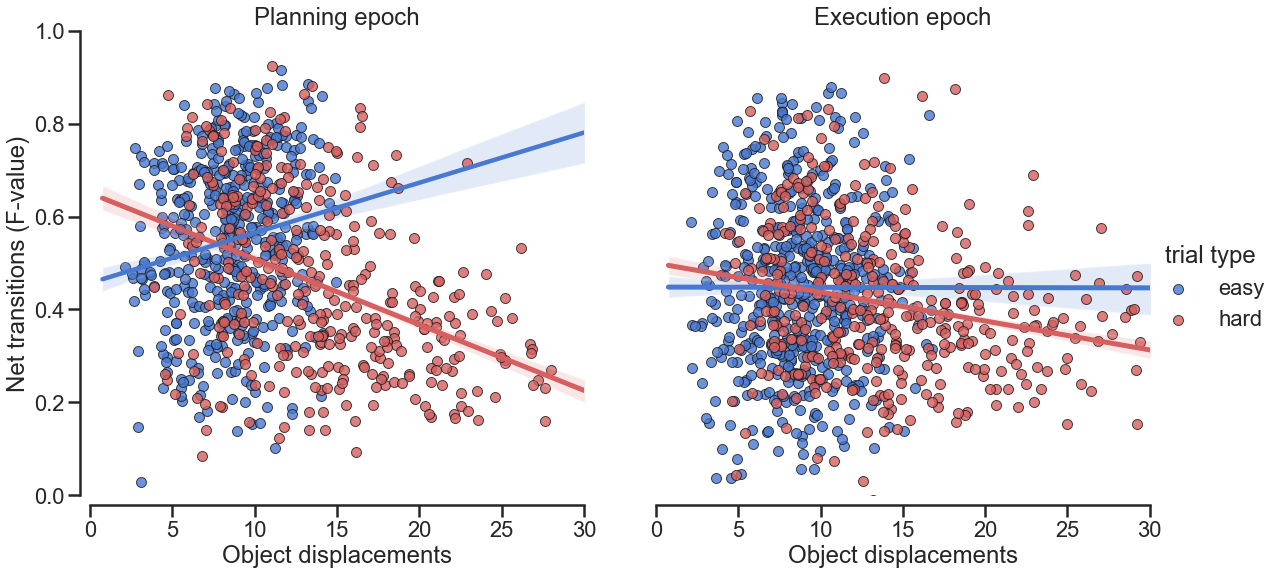
\includegraphics[width=0.9\linewidth]{source/figures/results/gaze_guidance_regression.png}
    \caption{Regression fit over the fixed-effects of trial types, epoch types and object displacements on the relative net transitions. Figure shows a scatter plot of the relative net transition (F-value) vs. number of object displacements per trial and differentiated for the two trial types EASY(blue), HARD(red). Each point refers to one trial and it's F value vs. the number of object displacements in that trial. The lines denote the regression fit and the shaded region denotes 95\% confidence interval.\\}
    \label{fig:F_regression}
\end{figure}

\begin{table}
\begin{tabular}{lrrrrrl}
\toprule
                                     factor &    Est &    SE &     LL &     UL &      Z &  Pvalue \\
\midrule
                        trial type &  0.124 & 0.024 &  0.076 &  0.171 &  5.061 &   0.000 *** \\
                              epoch type &  0.081 & 0.024 &  0.034 &  0.128 &  3.389 &   0.001  ***\\
                                  object displacements & -0.003 & 0.001 & -0.005 & -0.001 & -2.611 &   0.009 ** \\
           trial type:epoch type &  0.145 & 0.048 &  0.051 &  0.239 &  3.019 &   0.003  **\\
               trial type:object displacements & -0.015 & 0.002 & -0.020 & -0.011 & -6.782 &   0.000 *** \\
                    epoch:object displacements &  0.001 & 0.002 & -0.003 &  0.006 &  0.635 &   0.526        \\
 trial type:epoch type:object displacements & -0.019 & 0.004 & -0.028 & -0.010 & -4.321 &   0.000 *** \\
\bottomrule
\end{tabular}
\\\\
\caption{\label{tab:lm_res}Model coefficients of the linear fixed effects model.}
\end{table}


Finally, the analysis above tells us the gaze scan paths and attention guidance behavior to and from relevant ROIs. However, it does not illustrate the primacy of ROIs based on selection by gaze. Even though there are higher proportion of fixations on the current\_TO and current\_TS during action execution, we cannot determine which ROIs were first fixated on during the action the execution epochs. Hence, we were further interested in finding the attention attraction of power of the ROIs. In the case of planning epochs if the first fixation on current\_TO is earlier than other ROIs, then the target location of the object is selected first and kept in memory while scanning other objects. If however, the first fixation on the current\_TO is latest in the sequence of ROIs, it signifies a search process conducted at start of action planning epoch where the eyes search for the appropriate location to place the object, "finds" it and performs the action execution. This would signify a just-in-time strategy of fixating on ROIs as and when they are needed for an action. Similarly, in the action execution epochs, if the first fixation on current\_TS is earlier than other ROIs, then the target location of the object is selected first and then other objects are scanned. If however, the first fixation on the current\_TS is latest in the sequence of ROIs, it signifies a search process conducted at start of action execution epoch and once the target shelf is located the action is terminated. 

As the action planning and execution epochs varied in duration, we normalized the time points by dividing them by the duration of the epoch. This way, time elapsed since start of epoch is comparable to all epochs across trials and subjects. To estimate the time elapsed until first fixation on the ROIs, we used a measure known as T50 which estimates the median (50\% quantile) time till first fixation on each of the 7 ROIs per trial. Hence, with multiple action execution epochs per trial, we estimate the T50 for each of the 7 ROI per trial. \textcolor{Blue}{Figure \ref{figure:t50_sub_plan}} shows the distribution of T50 over the 7 ROIs in the action planning epochs. As the shown in the figure, there are early re-fixations on the the prev\_TS and prev\_TO as the gaze moves away from right after completing the previous action execution epoch followed by fixations on 'other' non-task relevant objects. In the later part of the epoch, T50 of first fixations on next\_TO, next\_TS and current\_TS are close together. More importantly, T50 for the current\_TO the shelf location where the target object is placed is last in the epoch after 50\% of the epoch time has elapsed. The results above have to be accounted for given the proportion of occurrence of the ROIs within a trial. As shown in \textcolor{Blue}{Figure \ref{figure:t50_plan_fix_prop}}, current\_TO and 'other' account for more than 50\% of the first fixations in the trial. Less than 1/10th of the fixations in a trial  are devoted to next\_TO, next\_TS and current\_TS.

\textcolor{Blue}{Figure \ref{figure:t50_sub_exe}} shows the distribution of T50 over the 7 ROIs. As the shown the figure, there are early re-fixations on the the current\_TO right after the onset of the action execution epoch followed by fixations on 'other' non-task relevant objects. In the later part of the epoch, T50 of first fixations on prev\_TO, prev\_TS, next\_TO and next\_TS are close together. More importantly, T50 for the current\_TS the shelf location where the target object is placed is last in the epoch after 50\% of the epoch time has elapsed. The results above have to be accounted for given the proportion of occurrence of the ROIs within a trial. As shown in \textcolor{Blue}{Figure \ref{figure:t50_exe_fix_prop}}, current\_TO and current\_TS account for more than 50\% of the first fixations in the trial, shortly followed by 'other' ROI. prev\_TO, prev\_TS and next\_TO, next\_TS comprise of less that 1/10th of the first fixations within a trial. This is an important caveat to note while assessing the T50 values for the ROIs where the T50 estimates for prev\_T0, prev\_TS, next\_TO, and next\_TS are based on small proportion of occurrences in a trial.

Taken together, this is further evidence of the a just-in-time strategy of gaze guidance during both action planning and execution epochs, where a "search" process is initiated for the current target object and shelf, with the search "ending" on the target object/shelf and immediately following an action of picking up the object or dropping it off. Most importantly, the latency of the fixation on the the current target object shows that object selection for action execution is not necessarily planned. In the action execution epochs, the latency of the T50 for the previous task related object and shelf show that a monitoring of the current action with respect to the previous action are at play, where fixations made to the prev\_TO and prev\_TS are made to confirm the choice of the current target shelf and might serve as look-back fixations. Further more, the latency of first fixations on the next task object close to the current target shelf indicates that in the 1/10th of the instances, gaze is used to pre-plan the next action before the end of the current action and might function as look-ahead fixations.

\begin{figure}[h]
    \centering
    \subfloat[]{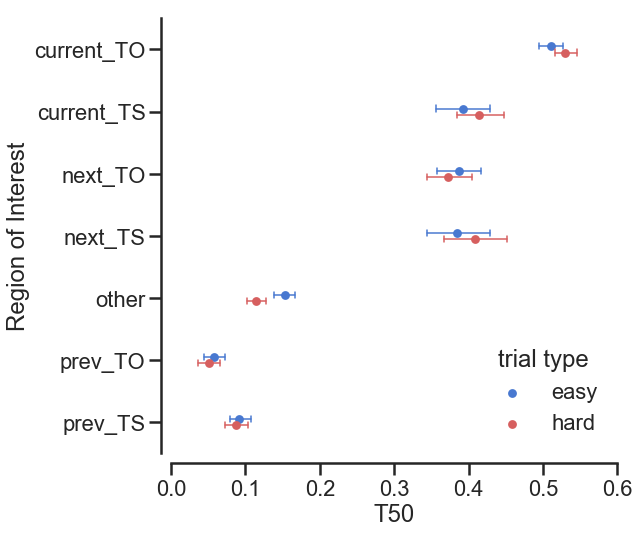
\includegraphics[width=0.3\linewidth]{source/figures/results/t50_subject_planning.png}
    \label{figure:t50_sub_plan}}
    \subfloat[]{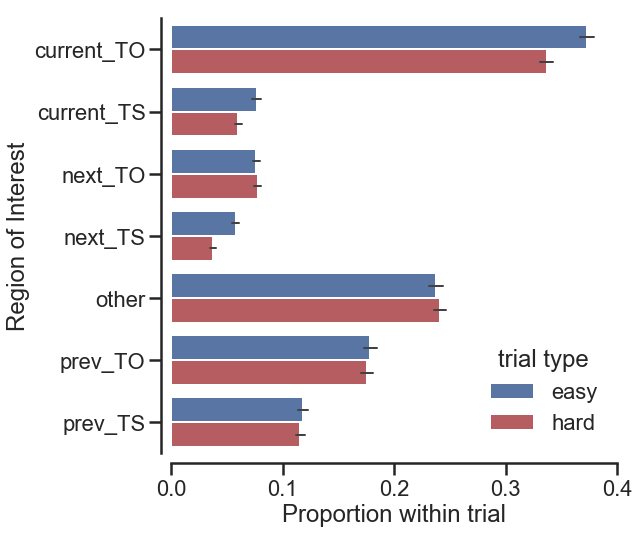
\includegraphics[width=0.3\linewidth]{source/figures/results/first_fix_roi_planning.png}\label{figure:t50_plan_fix_prop}}
    \caption[]{T50 for the action planning epochs. In order to capture the latency T50 as an estimator for latency of first fixation on the 7 ROIs per trial.
    Panel \protect\subref{figure:t50_sub_plan} shows the mean and 95\% confidence interval of T50 estimate for each trial. Blue points show the mean T50 for EASY trials and red points show the the T50 for the HARD trials.
    Panel \protect\subref{figure:t50_plan_fix_prop} shows the proportion of first fixations on each of the 7 ROIs in the planning epochs within a trial. Blue bars show proportion of first fixation on given ROI for EASY trials, red bars for HARD trials. Error bars indicate 95\% confidence interval. }
     \label{figure:t50_subject_plan}
\end{figure}

\begin{figure}[h]
    \centering
    \subfloat[]{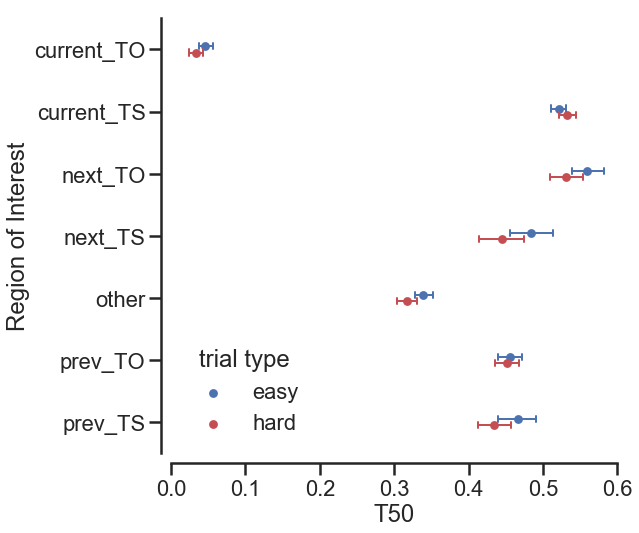
\includegraphics[width=0.3\linewidth]{source/figures/results/t50_subject_execution.png}\label{figure:t50_sub_exe}}
    \subfloat[]{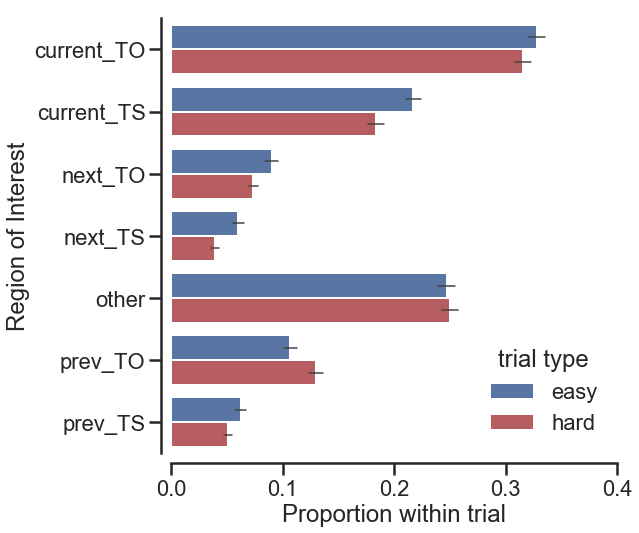
\includegraphics[width=0.3\linewidth]{source/figures/results/first_fix_roi_execution.png}\label{figure:t50_exe_fix_prop}}
    \caption[]{ T50 for the action execution epochs. In order to capture the latency T50 as an estimator for latency of first fixation on the 7 ROIs per trial. 
    Panel \protect\subref{figure:t50_sub_exe} shows the mean and 95\% confidence interval of T50 estimate for each trial. Blue points show the mean T50 for EASY trials and red points show the the T50 for the HARD trials.
    Panel \protect\subref{figure:t50_exe_fix_prop} shows the proportion of first fixations on each of the 7 ROIs. Blue bars show proportion of first fixation on given ROI for EASY trials, red bars for HARD trials. Error bars indicate 95\% confidence interval.
    }
    \label{figure:t50_subject_exe}
\end{figure}